\subsection{Suprema and infima in an ordered group}

Recall (Set Theory, III, p.~141) that if the set of upper bounds of a subset \(F\) of an ordered set \(E\) (that is to say the set of \(z \in E\) such that \(x \leqslant z\) for all \(x \in F\) ) has a least element \(a\) , then this element, which is then unique, is called the supremum of \(F\) . If \(F\) is the set of elements in a family \((x_{i})_{i \in I}\) of elements of \(E\) , its supremum, if it exists, is denoted \(\sup_{i \in I} x_i\) (or \(\sup_{i} x_i\) or simply \(\sup(x_i)\) ); if it is a

finite family \((x_{\iota})\) \((1 \leqslant \iota \leqslant n)\) , this supremum is also denoted sup \((x_{1}, \ldots, x_{n})\) . The infimum is defined in an analogous manner and is denoted inf. The operations sup and inf are associative and commutative.

Recall (Set Theory, loc. cit.) that if F is a subset of an ordered set E, and \((x_{t})\) a family of elements of F, then the existence of \(\sup(x_{t})\) in E (which may be denoted \(\sup_{E}(x_{t})\) ) does not imply the existence of a supremum of the \(x_{t}\) in F (which may be denoted \(\sup_{F}(x_{t})\) when it does exist); if both exist we know only that \(\sup_{E}(x_{t}) \leqslant \sup_{F}(x_{t})\) ; however if \(\sup_{E}(x_{t})\) exists and belongs to F, then \(\sup_{F}(x_{t})\) exists and is equal to \(\sup_{E}(x_{t})\) . For example, in the polynomial ring A = K{[}X, Y{]} (K a field), the principal ideals AX and AY have the ideal AX + AY as supremum (under the relation ⊂) in the ordered set of ideals of A, but have the ideal A as supremum in the set of all principal ideals of A.

(DIV) An element \(d\) of \(\mathbf{K}^*\) is called a greatest common divisor, or gcd for short, of a family \((x_{\iota})\) of elements of \(\mathbf{K}^*\) , if the principal fractional ideal \((d)\) is the supremum in \(\mathcal{P}^*\) (under the relation \(\subset\) ) of the family of ideals \(((x_{\iota}))\) , or in other words if the relation \(z \mid d\) for \(z \in \mathbf{K}^*\) is equivalent to \(\ll z \mid x_{\iota}\) for all \(\iota\) ». In the same way we will say that \(m \in \mathbf{K}^*\) is a least common multiple or an lcm of the family \((x_{\iota})\) if \((m)\) is the infimum in \(\mathcal{P}^*\) of the family of ideals \(((x_{\iota}))\) , that is if \(m \mid z\) is equivalent to \(\ll x_{\iota} \mid z\) for all \(\iota\) . It amounts to the same thing to say that \((m) = \bigcap_{\iota} (x_{\iota})\) ; indeed, the condition \(x_{\iota} \mid z\) for all \(\iota\) is equivalent to \(z \in Ax_{\iota}\) for all
\(\iota\) , that is to \(z \in \cap (x_{\iota})\) , and the condition \(m \mid z\) is equivalent to \(z \in (m)\) \(^{1}\) .

\pandocbounded{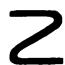
\includegraphics[keepaspectratio]{images/part002_2ca33fff.jpg}}

Note that if a principal fractional ideal \((d)\) satisfies \((d) = \sum_{i} (x_i)\) then \(d\) is a gcd of the family \((x_{\iota})\) ; but conversely a gcd of \((x_{\iota})\) does not necessarily satisfy the above condition (cf.~VI, p.~33, Ex. 24).

The gcd and lcm, if they exist, are well defined modulo the subgroup U of units of \(K^{*}\) , that is two gcd's (or two lcm's) of a given family are associate; by abuse of language we will often write \(\gcd(x_{t})\) and \(\operatorname{lcm}(x_{t})\) for any of the gcd's or lcm's of the family \((x_{t})\) , whenever such elements exist.

(DIV) By abuse of language we sometimes extend the notion of gcd to a family \((x_{i})\) of elements of K, some of which may be zero; this gcd is again defined to be an element d such that the relation \(z \mid d\) is equivalent to « \(z \mid x_{i}\) for all \(i\) »; clearly d is 0 if all the \(x_{i}\) are zero; otherwise d is a gcd of the nonzero \(x_{i}\) . Similarly the lcm of a family, some elements of which are zero, is 0.

In an ordered group G, an immediate consequence of the invariance under translation of the ordering (VI, p.~2, Prop. 2) is that

\[
\sup \left(z + x _ {i}\right) = z + \sup \left(x _ {i}\right)\tag{1}
\]

in the sense that, whenever one side is defined, then so is the other and the two are equal. Similarly, it follows from the fact that the map \(x \mapsto -x\) takes the ordering of G to the opposite ordering (VI, p.~3, Cor.) that

\[
\inf (- x _ {i}) = - (\sup (x _ {i})),\tag{2}
\]

this relation being understood in the same sense as the previous one.

PROPOSITION 6. --- Let \((x_{\alpha})_{\alpha \in A}, (y_{\beta})_{\beta \in B}\) be two families of elements of an ordered group G, each having a supremum. Then the family \((x_{\alpha} + y_{\beta})_{(\alpha, \beta) \in A \times B}\) has a supremum, and \(\sup_{(\alpha, \beta) \in A \times B} (x_{\alpha} + y_{\beta}) = \sup_{\alpha \in A} x_{\alpha} + \sup_{\beta \in B} y_{\beta}\) .

Indeed, from \(x_{\alpha} + y_{\beta} \leqslant z\) for all \(\alpha\) and \(\beta\) , we deduce \(\sup (x_{\alpha}) + y_{\beta} \leqslant z\) for all \(\beta\) , and hence \(\sup (x_{\alpha}) + \sup (y_{\beta}) \leqslant z\) .

